\section{Ergänzungen zur Analyse}

\subsection{Omni-Outliner}

\medskip
\begin{figure}[ht] 
  \begin{center}
    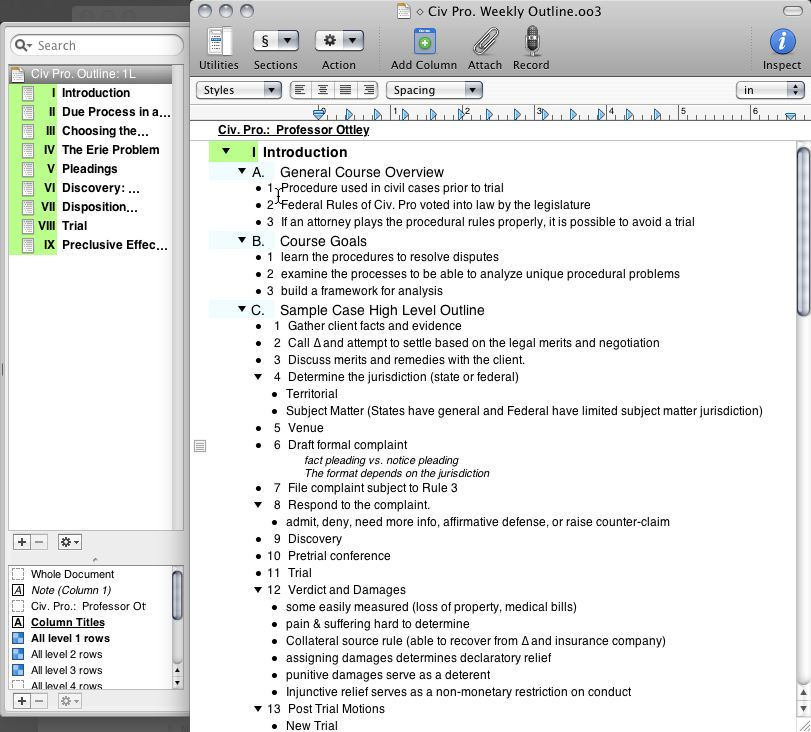
\includegraphics[width=\textwidth]{grafik/omnioutliner-screenshot} 
  \end{center}
  \caption{Screenshot von OmniOutliner \cite{omnioutliner:screenshot}}
  \label{fig:omnioutliner-screenshot} 
\end{figure}



\subsection{Der Hype-Zyklus von Gartner}
\label{subsec:hype-cycle}

Aus dem Hype-Zyklus sind die Phasen der öffentlichen Aufmerksamkeit ablesbar, die eine neue Technologie nach ihrer Einführung durchläuft. Die X-Achse bezeichnet die Zeit nach der Einführung, die Y-Achse die Aufmerksamkeit für die Technologie. 

\medskip
\begin{figure}[H] 
  \begin{center}
    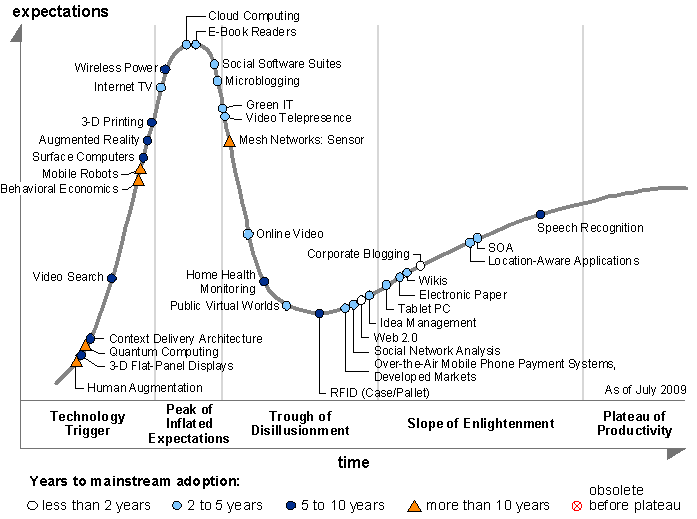
\includegraphics[width=\textwidth]{grafik/gartner-hype-cycle-2009} 
  \end{center}
  \caption{Hype-Zyklus von Gartner 2009, \cite{cloud:hypecycle}}
\end{figure}


